\documentclass[a4paper]{article}
\usepackage[margin=1in]{geometry} 
\usepackage{graphicx}
\usepackage{wrapfig}
\usepackage{url}
\usepackage{multirow}

\title{Peptide retention time prediction} 


\author{
Luminita Moruz\\
Science for Life Laboratory,\\
School of Biotechnology,\\
Royal Institute of Technology (KTH),\\
Stockholm, Sweden
\and
Lukas K\"{a}ll\\
Science for Life Laboratory,\\
School of Biotechnology,\\
Royal Institute of Technology (KTH),\\
Stockholm, Sweden}


\begin{document}

\maketitle

\setcounter{secnumdepth}{2} % organisational level that receives a numbers
\setcounter{tocdepth}{2}    % print table of contents for level 2
\tableofcontents            % print the table of contents
% levels are: 0 - chapter, 1 - section, 2 - subsection, 3 - subsubsection

\setlength{\parskip}{0.15cm}

\section{Introduction}

Mass spectrometry (MS) based methods are unquestionably the most
popular techniques for analyzing the protein content of biological
mixtures.  The ever-expanding palette of applications range from
identifying and quantifying proteins in biological samples
\cite{Geiger2012} to determining posttranslational modifications
\cite{Huttlin2010} and elucidating protein interaction networks
\cite{Gavin2011}.


Although available in a variety of flavors, most of the widely spread
MS-based workflows consists of the same main steps. First, the
proteins in the mixture of interest are cleaved into peptides using a
sequence-specific enzyme such as trypsin. This step is necessary
because the mass spectrometers are more sensitive for peptides, and
because spectra produced by full-length proteins are difficult to
interpret. In the next step, the resulting peptides are separated
according to their hydrophobicity on a liquid chromatography (LC)
column. As they gradually elute from the column, the peptides are
ionized via electrospray ionization and subjected to mass spectrometry
analysis. The result of these measurements consists of a set of
spectra, which are subsequently used to infer valuable information
about the proteins present in the initial sample.


Today a majority of the mass spectrometry (MS) protocols in use are
high-throughput, generating extensive amounts of data. This has
brought up a whole new set of analytical challenges, making the
development of efficient algorithms to interpret this data a major
area of proteomics research. A particular difficult challenge in this
context is posed by the tremendous complexity of the data. Proteins
display a wide range of physico-chemical properties and are often
found at very different amounts in complex samples, spanning as much
as 12 orders of magnitude in relative abundance~\cite{Angel2012}.
Furthermore, a large proportion of proteins are subjected to
posttranslational modifications~\cite{Lemeer2009}. To manage this
formidable diversity, increasing efforts are made to extract besides
the fragmentation spectra additional information from each MS
experiment.

An example of such additional information is represented by retention
times, i.e. the time points when peptides elute from the liquid
chromatography column.  The main purpose of liquid chromatography is
to reduce the number of peptides simultaneously injected into the mass
spectrometer. This increases the probability of each individual
peptide to be selected for fragmentation, which in its turn, increases
the proteome coverage achieved in an experiment.  However, besides
this, the separation process in itself provides useful information
about the analytes. On the one hand, the instrument always records the
time when a peptide elutes from the chromatography column, i.e. the
retention time. On the other hand, the retention time can also be
estimated by examining the sequence of the peptide. The availability
of both predicted and observed retention times has proven to be a
powerful feature, with several applications in MS-based proteomics
\cite{Palmblad2013}.


In this review we summarize the work done in the field of retention
time prediction, and describe a few of the successful applications of
such predictions. Sections~\ref{sec:rtpred} and \ref{sec:rtpredm}
describe the main approaches to retention time predictions from
peptide sequences. Section~\ref{sec:app} discusses some of the most
important applications of retention time predictions.
% Section~\ref{sec:irt} briefly introduces the use of peptide retention
% standards.


\section{\label{sec:rtpred}Retention time prediction for unmodified peptides}


Liquid chromatography gives reproducible results. Except for small
shifts from run to run, the same peptide elutes at about the same time
when a sample is reanalyzed under identical experimental conditions
(Figure~\ref{fig:repr}). This suggests that peptides engage in
well-defined interactions during separation, which depend only on the
experimental setup employed and the properties of the peptides
themselves. However, the properties of the peptides are determined to
a large extent by their amino-acid sequence. As a consequence, given a
chromatography setup, the sequence of a peptide should provide
virtually all the information needed to predict its retention time.

\begin{wrapfigure}{r}{.45\textwidth}
\vspace{-10pt}
%\begin{figure}[htbp]
\centering
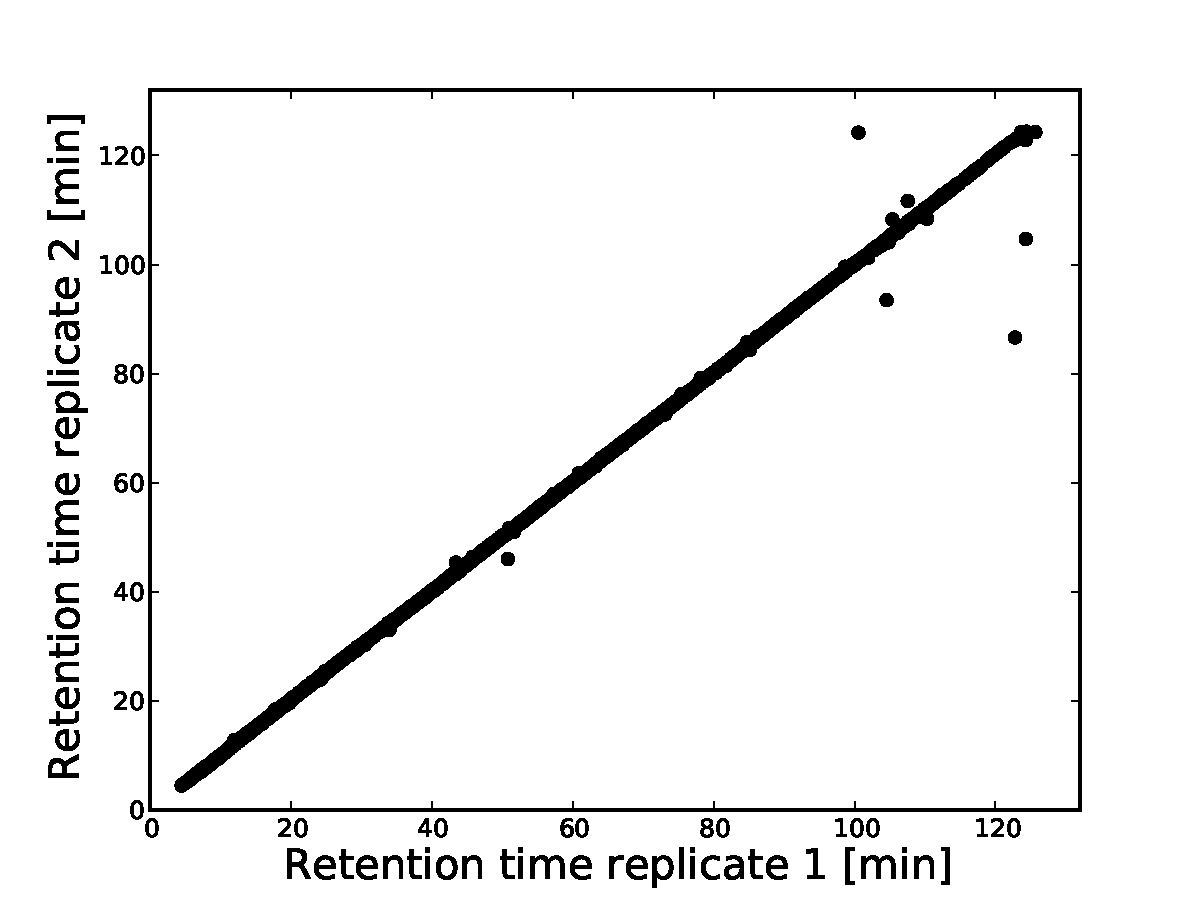
\includegraphics[trim=0.5cm 0cm 2cm 1.5cm, clip=true, width=0.43\textwidth]{img/reproducibility.pdf}
\caption{\label{fig:repr} {\bf Reproducibility of peptide retention time.} Two identical shotgun proteomics experiments were carried out. The retention times of the peptides confidently identified in both runs are displayed.}
%\end{figure}
\vspace{-25pt}
\end{wrapfigure}

% iRT? \cite{Escher:2012qv}
Following these observations, a variety of retention time prediction
methods has been proposed. Most naturally one could divide these
methods into four classes: look-up tables-based approaches,
index-based methods, modeling-based methods and machine learning
techniques. The main ideas underlying each category are described
below, while Table \ref{tab:rtmethods} lists a few of the most popular
retention time prediction methods from each category.

\subsection{Methods based on look-ups of previous registered retention times}

These methods involve keeping a database of previously observed
retention times for a set of peptides, and subsequently use these
values as a basis for retention time predictions. In particular, in
the past years the use of retention standards has become increasingly
widespread \cite{olegstd, irt}. Such standards typically consist of a
small number of peptides covering a wide span of hydrophobicities and
favorable for detection by mass spectrometry. These peptides are often
analyzed together with the sample of interest, and by comparing their
observed and expected behaviors one can obtain valuable information
for a variety of applications.

\vspace{0.15cm}

As an example, in targeted proteomics, peptide standards can be used to
 calibrate predicted retention times and to estimate the accuracy of
 the prediction algorithms~\cite{Kiyonami01022011}. In addition,
 recent studies have reported excellent results when using peptide
 standards to adjust the time when certain transitions are scheduled
 ``on-the-fly''~\cite{seb, irt}. Retention standards are also useful
 for aligning data from multiple experiments~\cite{petritis2003}, to
 transfer retention times between different chromatography
 setups~\cite{seb}, or to keep track of the performance of LC-MS/MS
 systems~\cite{qcal}.

\subsection{Index-based methods}
\label{sec:irt}
\hyphenation{lear-ning}
\hyphenation{indivi-dual}

% Basic idea 
Index-based prediction methods aim at estimating the effect that each
individual amino acid in a sequence has on the retention time of the
peptide. The individual contributions of the amino acids are often
referred to as retention coefficients, and a set of retention
coefficients forms a retention index. Once a retention index is
derived for a given chromatography system, the retention time of a
peptide can be estimated by simply summing up the retention
coefficients of the constituent amino acids.

% The first method 
The first method to implement this idea used a set of 25 short
peptides together with their observed retention times to derive
retention coefficients for each of the amino acids and end groups
present in the sequences \cite{meek1980}. The coefficients were
calculated using a form of iterative regression and were estimated
using only the amino-acid composition of the peptides, without any
information about the position of each amino acid in the
sequence. However, since shuffled versions of the same peptide
sequence had previously been separated on a RPLC column, the author
pointed out that additional parameters would be required for
predicting the retention time of longer peptides.


\begin{table}
 \caption{{\bf Retention time prediction methods.} We
   give a few of the most commonly used retention time prediction methods available.}
 \vspace{.2cm}
 \label{tab:rtmethods}
 \begin{tabular}{lll}

 Method name & Link & References  \\
 \hline
SSRCalc & \url{http://hs2.proteome.ca/SSRCalc/SSRCalcX.html} & \cite{Krokhin2004, Krokhin2006}, \cite{Spicer2007} \\
BioLCCC & \url{http://theorchromo.ru/} & \cite{gorshkov2006} \\
ANN & Link? & \cite{petritis2003,petritis2006improved} \\
RTModel, RTPredict &  \url{http://ftp.mi.fu-berlin.de/OpenMS/documentation/html/TOPP_RTPredict.html}, 
 & \cite{rtpredict, rtpredictImproved} \\
&\url{http://ftp.mi.fu-berlin.de/OpenMS/documentation/html/TOPP_RTModel.html}  & \\

Elude & \url{http://elude.sbc.su.se/} & \cite{elude1, elude2} \\
iRT-calculator & http://www.biognosys.ch/products/irt-calculator.html
& \cite{irt} \\
\hline
 \end{tabular} \\
\end{table}

%The study reported good correlations between predicted and observed
%retention times, showing that for short peptides the amino acid
%composition provided sufficient information to produce reasonable
%retention time predictions.



% It became available that additional information is needed; anc oclumn is important  examples 
Indeed, a subsequent study showed that even for short peptides,
distinct retention coefficients are obtained when an amino acid is
located at different positions in a sequence \cite{Houghten1987}. In
this context, the authors speculated that different retention
coefficients would be needed for each position in a peptide
sequence. Although the exact chemical mechanisms underlying this
observation are still not fully understood, a number of studies have
pinpointed individual factors that alter the retention coefficients of
amino acids. As an example, it has been shown that the retention
contribution of an amino acid is affected by the overall
hydrophobicity of the peptide \cite{Mant2006}, the number of positive
charges \cite{Mant2006} or presence of elements of secondary
structure \cite{Zhou1990}. In addition, modifications in
chromatography setup such as changing the composition of the mobile or
stationary phases also modify the elution pattern of the
peptides \cite{Browne1982, Guo1987, Gilar2010}.


% SSRcalc was proposed including a number of additional terms; then it was extended
% for a few other column
Following these observations, Krokhin et al. developed SSRCalc
\cite{Krokhin2004}, which is currently the most widely used
index-based retention time predictor. In the initial version of the
algorithm a collection of 346 tryptic peptides was used to derive two
sets of retention coefficients, one corresponding to the N-terminal
and one to all the other positions in a peptide sequence. Furthermore,
correction factors for peptide length and overall hydrophobicity were
included. Subsequent versions of the algorithm included terms
accounting for additional properties such as isoelectric point,
nearest-neighbor effects of charged peptides and propensity to form
helical structures \cite{Krokhin2006}. Recently, it was showed that
interactions involving helical structures are highly complex, and thus
more sophisticated models are needed to account for the effects that
such interactions have on peptide retention time \cite{ah}.

A limitation of index-based methods are that they are optimized for
predicting retention times for certain chromatography setups. Thus,
their prediction ability deteriorates for experimental conditions
diverging from the setup on which the algorithm was optimized
\cite{Spicer2007}.

% - sum of retention coefficients (Meek reference 22) - different RT
% coefficients and the observation that this coefficients depend on
% the chromatography system (Browne ref 24) - investogate the
% contribution of individual amino acids (Guo 26,27) - all the work
% above was done on synthetic peptides os simple samples. Then RT
% prediction for complex sa% mples was proposed by (Palmblad 28-30) -
% important the exact position of each aa (pref 27) - additional rules
% included peptide length (ref 32), position of K and R residues [ref
% 33], and in the e% nd that the position of each amino acid at each
% position is important [ref 34] - amphipathicity [ref 35] - SSRCalc
% [ref 36-39]


\subsection{Modeling-based approaches}

Modeling-based techniques predict retention times by using information
about the structure of the peptides and/or their chemical interactions
during separation. An example is the methods based on Quantitative
Structure-Retention Relationships (QSRR) \cite{Kaliszan2005,
Baczek2005}. In such approaches specialized molecular modeling
software is used to calculate a number of chemical descriptors from
the peptide sequence. The most relevant such descriptors are then
selected and combined via regression analysis into a prediction
function, which is subsequently used to estimate retention time for
other peptides of interest.



In other modeling-based approaches theoretical models are used to
capture the chemical behavior of peptides on the chromatography
column. One such method is BioLCCC, which attempts to model the
connectivity of the amino acids in a peptide chain and the general
mechanisms of chromatographic
separation \cite{gorshkov2006}. Nevertheless, given the numerous
factors involved in peptide separation, modeling approaches often
involve a considerable number of simplifications.

 
\subsection{Machine learning-based methods}

In machine learning-based approaches a set of training peptides,
i.e. peptide sequences with known retention times, are used to
customize a predefined mathematical model. This step is typically
called training or learning. Once trained, the mathematical model can
be subsequently used to predict retention time for other peptides of
interest.


One of the first machine learning approaches for retention time
prediction was based on an Artificial Neural Network
(ANN) \cite{petritis2003}. Initially, each peptide was described by 20
features giving the number of each of the 20 amino acid residues
present in the sequence. The network was trained using $\sim$7000
peptides with known retention times and evaluated using a set of
$\sim$5000 peptides originating from another organism. The algorithm
reported good accuracy, especially taking into account that it only
used information about the amino acid composition of the peptides.



In a follow-up work, the method was extended by representing each
peptide by 1052 instead of 20 features
\cite{petritis2006improved}. The new descriptors encoded the identity
of each amino acid at each position in a sequence, as well as the
length and the hydrophobic moment of the peptide. The new neural
network was trained on more than 300,000 peptide sequences. To obtain
such a large number of peptides with known retention times, a strategy
to normalize elution times was developed. This allowed pooling of
peptides identified in more than 12,000 shotgun experiments. The
trained algorithm reported excellent performance for the 1303 peptides
on which it was evaluated.



A drawback of the method was however the large amount of training
peptides required, which made the algorithm difficult to retrain for
other chromatographic conditions. This was a serious limitation in the
context of RPLC separation, where a broad variety of chromatographic
setups is commonly used across research laboratories. To address this,
Klammer et al. proposed a predictor based on support vector machines
(SVMs) \cite{klammer2007improving}. Their method required fewer
training peptides and could thus be easily adapted to new
chromatographic conditions, but yielded lower prediction
accuracy. Subsequently, a more elaborate SVM-based method using a
customized kernel function was proposed \cite{rtpredict, rtpredictImproved}. This
approach provided reasonable prediction accuracy, while requiring as
little as 50 peptides for training.

% Other retention time prediction method used a feature selection
% approach to select relevant descriptors, and showed good
% performances even for longer peptides containing up to 50 amino
% acids \cite{shinoda2006}.



Moruz {\em et al.} developed a software package for retention time
prediction which we named {\sc Elude} \cite{elude1, elude2}. One of
the main novelty points of {\sc Elude} was the calculation of peptide
features based on both a general hydrophobicity index, as well as a
retention index trained for each dataset at hand. This ensured that
the algorithm could be applied to different chromatography setups with
minimal loss in performance. For cases when little training data was
available, {\sc ELUDE} implemented an additional workflow based on a
library of pre-trained retention models. This workflow required only a
few tens of training peptides to select and calibrate the most
suitable model from the library. Both the selection and calibration
were performed using statistical methods robust to outliers.



However, despite all these efforts, it should be pointed out that none
of the retention time prediction methods currently available is able
to provide accuracy comparable to the small shifts observed when
running a sample twice through a chromatography column
(Figure \ref{fig:repr}). Recently, the lack of suitable
representations for secondary structure elements was indicated as one
of the main causes of prediction errors \cite{Reimer2012}.  Most
probably additional factors are involved, and further endeavors are
required to reach the desired level of accuracy.

\section{\label{sec:rtpredm}Retention time prediction for modified peptides}

% very few studies have documented the chromatographic behavior of
% modified peptides
The study of peptide separation mechanisms in RPLC has been an active
area of research for the past 30 years. Nonetheless, surprisingly
little efforts have been directed toward investigating the
chromatographic behavior of posttranslationally modified peptides. The
few studies available so far have mostly focused on phosphorylated
peptides \cite{Kim2007}, or a couple of artifactual modifications
commonly introduced during sample
preparation \cite{Reimer2011}. Consequently, few retention time
prediction methods have been extended and assessed for such
peptides. A majority of the approaches currently available are
modification-specific, many of them developed specifically for
phosphopeptides \cite{Kawakami2005, perlova2010}.

\begin{figure}[!h]
\centering 
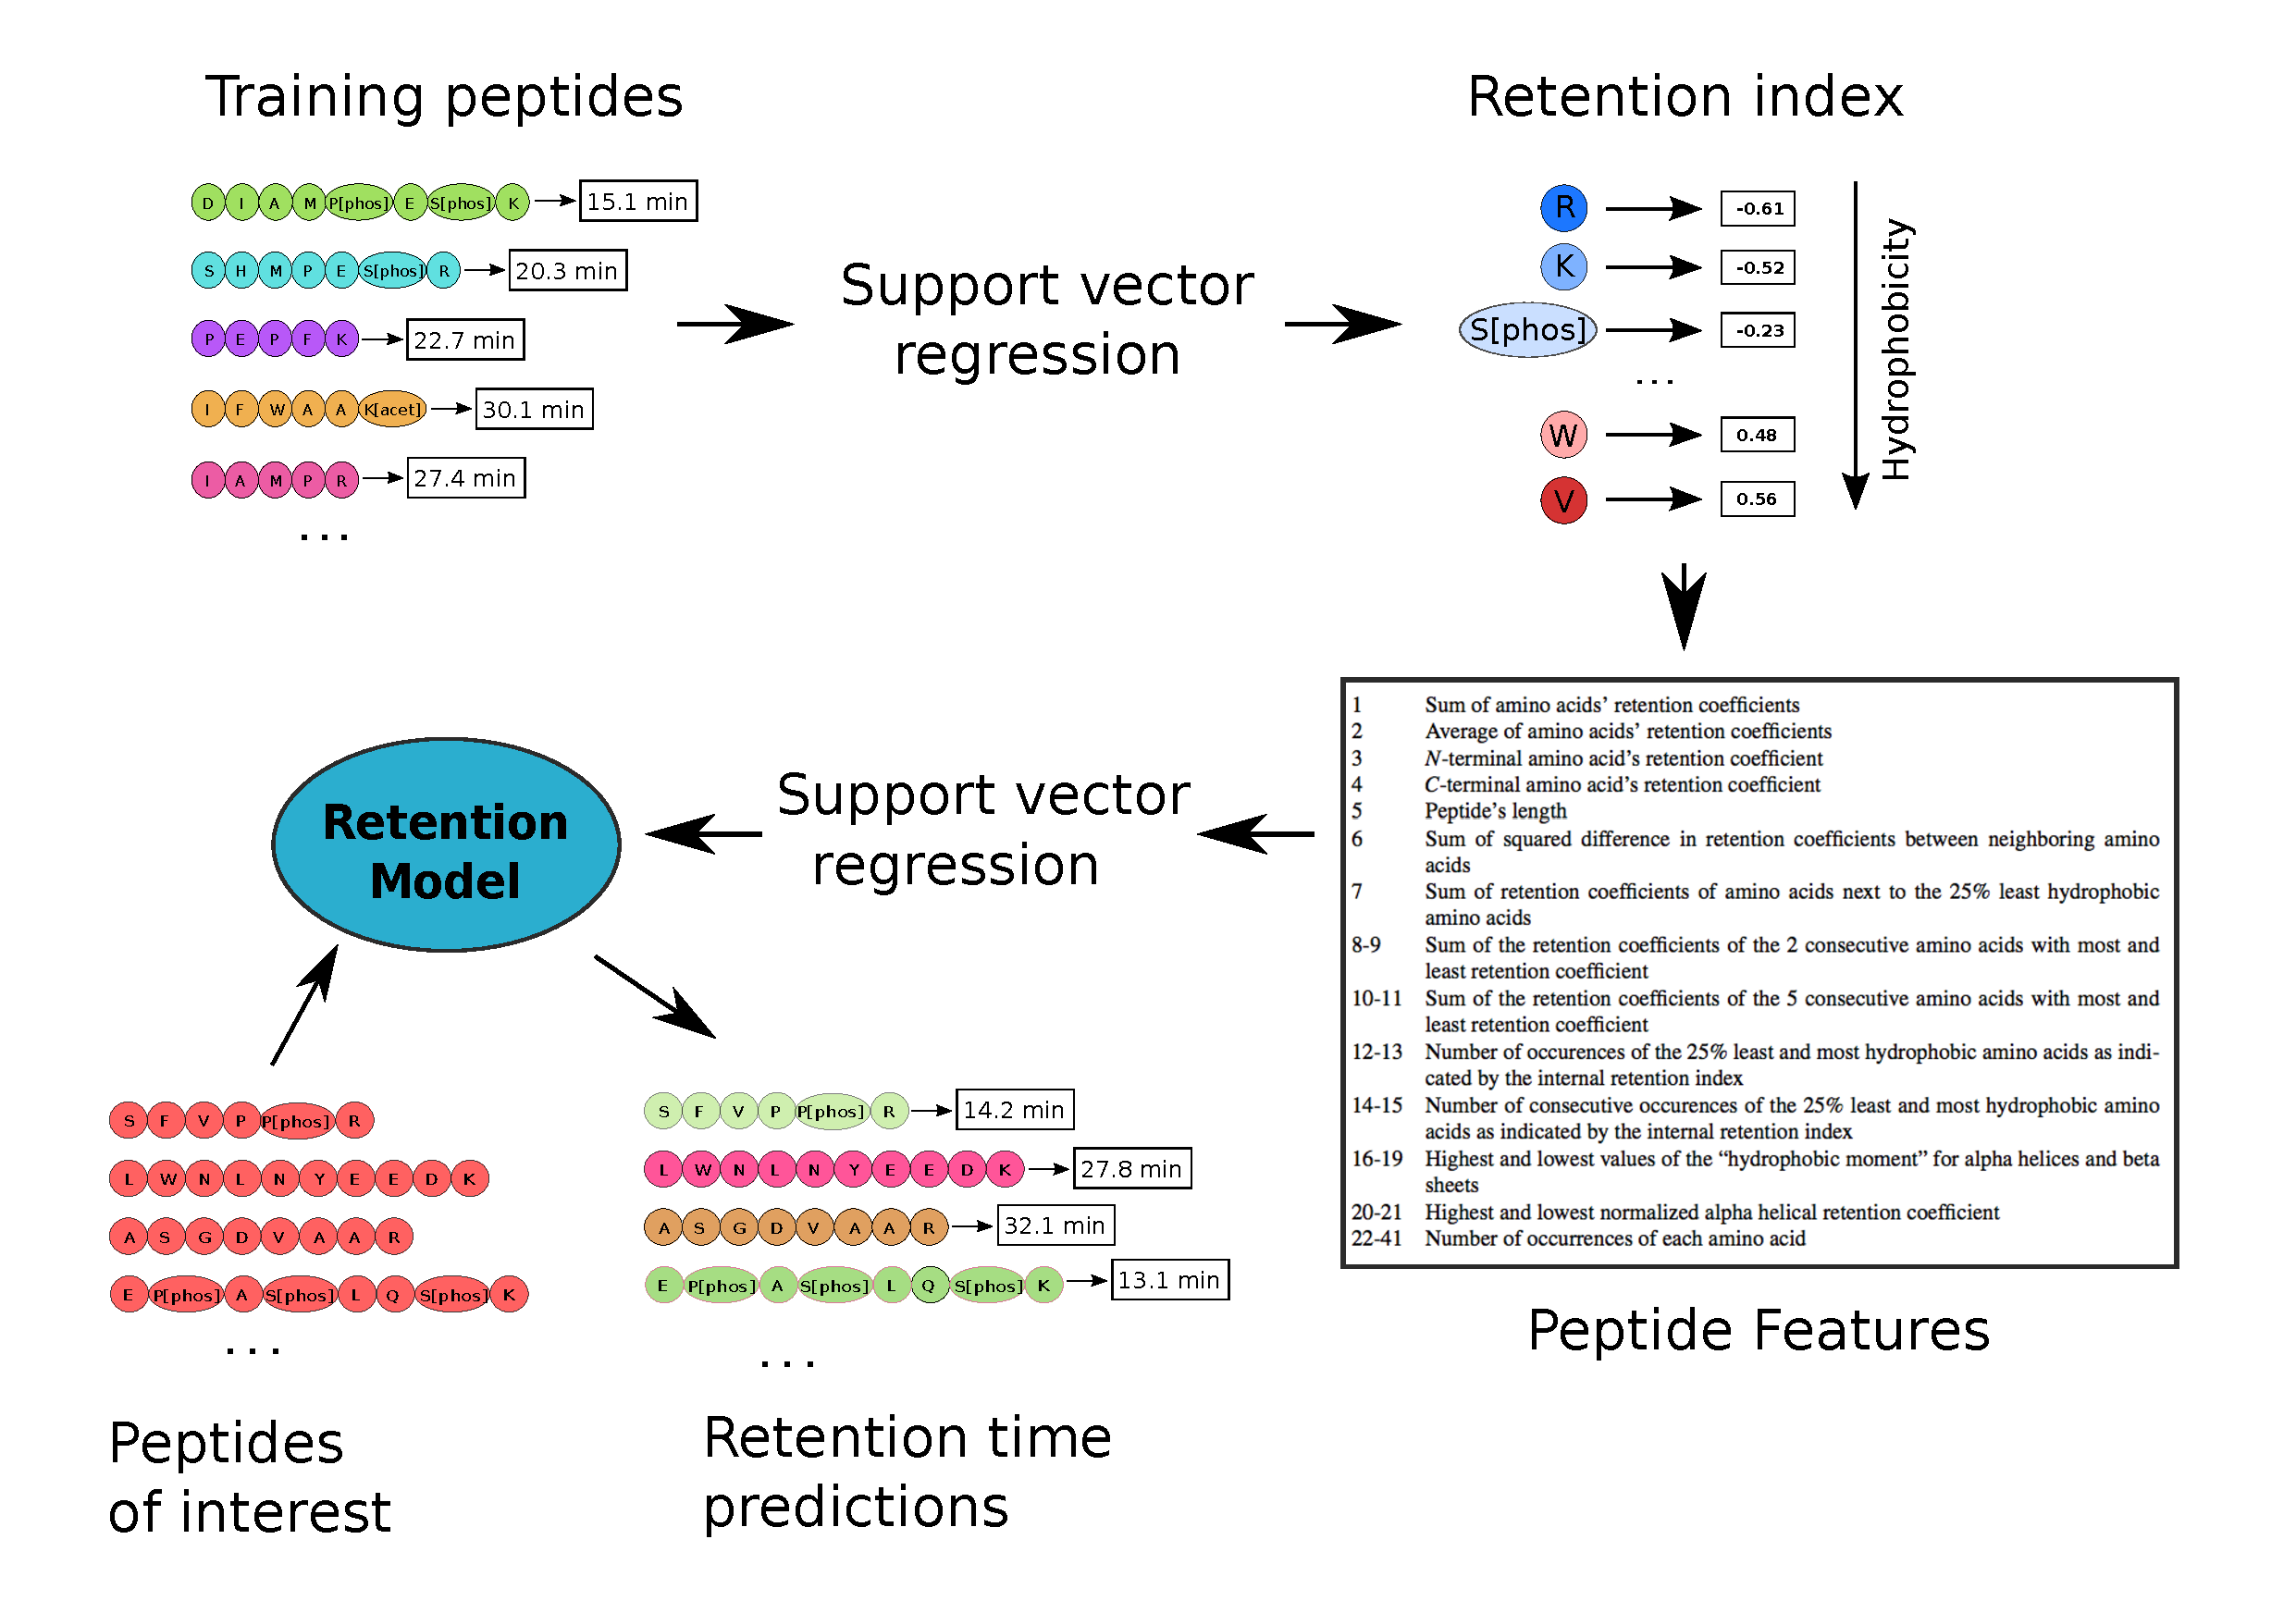
\includegraphics[width=0.9\textwidth]{img/elude-ptm.pdf}
\caption{\label{fig:elude} {\bf {\sc Elude}'s workflow.}  {\sc Elude} encompasses two learning steps. In the first one the training peptides are used to build an in-house retention index. This index, together with additional information, is then employed to calculate a set of 60 numerical features for each peptide. These features are optimally combined during a second training procedure. The resulting retention model can be subsequently used to predict the retention time of other peptides of interest.}
\end{figure}



To address this, in our group we extended the first version of our
algorithm {\sc ELUDE} to encompass modified peptides as well. This was
straightforward to achieve once we observed that the in-house trained
retention index contained nearly all the information incorporated in
the more general hydrophobicity scale. This meant that we could remove
all the features based on this index with minimal loss in
accuracy. Further, we redefined all features describing a peptide in
terms of the in-house retention index alone. Since this index was
trained for each dataset at hand, the algorithm became fully trainable
for any modified amino acid (Figure \ref{fig:elude}). We evaluated the
new version of {\sc ELUDE} on peptides containing artifactual
modifications introduced as part of an MS protocol called COmbined
FRActional DIagonal Chromatography (COFRADIC) \cite{Gevaert2002}. Our
results showed that {\sc ELUDE} yielded equally accurate predictions
for modified and unmodified peptides \cite{elude2}.

As large-scale studies of a variety of posttranslational modifications
increasingly come within reach, predictors
handling other modifications will become available. In this context,
machine learning methods are expected to play an important role
because of their flexibility and intrinsic ability to adapt to new
datasets.


\section{\label{sec:app}Applications of retention time prediction}

% RT prediction is used to increase number of identifications 
The time points when peptides elute from the RPLC column are typically
recorded in MS experiments. By comparing these values with predicted
retention times for peptides from a sequence database, information
about the identity of the peptides can be obtained. This relatively
straightforward idea has been implemented in a variety of flavors and
was proven to bring significant improvements in the peptide
identification process.


Palmblad {\em et al.} showed that matching theoretical and observed masses
and retention times provides a simple, yet powerful method to identify
peptides in simple biological
mixtures \cite{palmblad2002prediction}. Strittmatter et al. used
retention time as a parameter in a discriminant function that
differentiated between correct and incorrect peptide
identifications \cite{Strittmatter2004}. Following this approach, they
reported $\sim$9\% more confident peptide identifications in a typical
shotgun experiment. Along the same lines, Klammer et al. demonstrated
that for specific experimental conditions, just filtering out peptides
with large deviations between observed and predicted retention time
leads to up to 50\% more
identifications \cite{klammer2007improving}. 



Moruz {\em et al.} also investigated the possibility to use predicted
retention times to increase the throughput of proteomics
experiments. Their starting point was the observation that in typical
shotgun proteomics experiments only a small fraction of the detected
ions is fragmented, and thus used to identify peptides. The remaining
unfragmented ions are usually disregarded in the subsequent data
analyses. In the light of these observations, they investigated
whether we could use information encapsulated by unfragmented ions to
improve the protein inference in shotgun proteomics \cite{mf}.



% how it works and main results
More specifically, we matched observed masses and retention times of
unfragmented ions to predicted masses and retention times for the
theoretical peptides from an {\it in silico} digest. We built a
statistical framework to assign protein probabilities based on these
matches, and combined the results with the ones obtained by the
typical workflow based on fragmented ions. Following this approach, we
obtained up to 7\% more protein identifications at a fixed false
discovery rate threshold of 1\% \cite{mf}.



The idea of identifying proteins based on entire peptides, rather than
peptide fragments, is not new. In fact, this was the principle
underlying peptide mass fingerprinting, one of the first methods used
to identify proteins via mass spectrometry. However, when introduced
in the 90's, mass fingerprinting could not be applied to unequivocally
identify proteins in complex biological samples. Consequently, shotgun
proteomics has gained popularity instead. Nevertheless, with great
developments in instrumentation leading to sub-ppm mass accuracies,
the possibility of using mass fingerprinting-like methods came back to
attention~\cite{iamt1}. Our study showed how improved mass accuracies
and retention time predictions enable the use of unfragmented ions
even in the context of complex peptide mixtures. 



Krokhin et al. illustrated yet another route to employ retention time
predictions \cite{krokhin200612, McQueen2012}. They showed that
theoretical retention times and mass measurements can be used to
define lists of peptides belonging to already identified proteins. The
instrument can be instructed to avoid fragmenting these peptides, thus
decreasing the number of fragmentation events that need to be acquired
for identifying a set of proteins.



% Improve the design of SRM experiments 
In addition, predicted retention times are useful investigating
the elution properties of the peptides.  To illustrate this, we predicted the retention time of all the
theoretical peptides from an {\it in silico} digest of the human
proteome using  {\sc ELUDE}  \cite{elude1}. This exercise revealed a rather skewed
distribution, with a majority of the peptides eluting in only a small
portion of the chromatography run. This suggested that
the linear gradient typically used in liquid chromatography are sub-optimal, and that one should be able to replace such gradients with nonlinear functions that produce even
distributions of the peptides across runs.




We tested this hypothesis by calculating and evaluating
two types of nonlinear gradients \cite{gradopt1}. Our results showed that the new
gradients not only provided more uniform distributions of the
peptides, but also led to an increase in the number of peptide
identifications. In addition, they facilitated the identification of
different peptide species compared to the typical linear gradients. To allow the easy calculation of nonlinear gradients by any MS practitioner, we also implemented a user-friendly graphical user interface that can be downloaded free of cost \cite{gradopt2}. 
Seen from a general perspective, this showed that the gradient function is yet another parameter that researchers can alter
in their experiments, opening up a whole new range of potential
applications. 




Other examples of applications of retention time predictions include the optimization of  {\em de novo} targeted proteomic
assays \cite{bertsch2010}, as well as decreasing the
number of candidate peptides during database
searching \cite{lobas2013} and accurate simulations of MS-based
experiments \cite{bielow2011}.


%\begin{figure}[!h]
%\centering 
%\includegraphics[width=0.8\textwidth]{grad.pdf}
%\caption{\label{fig:svm} {\bf Workflow to calculate nonlinear gradients.} We calculated two types of nonlinear gradients: one that evens out the predicted distribution of the peptides from an {\it in silico} digest of the proteome, and one that uniformizes the distribution of the abundant MS1-ions.}
%\end{figure}

% It is an orthogonal information. Decrease the database search space,
% study properties of the peptides
 
%\section{\label{sec:irt}Peptide retention standards}

%\hyphenation{wide-spread}
% peptide standards what they are, what they are used for 
%In the past years, the use of retention standards has become
%increasingly widespread in the context of mass spectrometry-based
%proteomics~\cite{olegstd, irt}. Such standards typically consist of a
%small number of peptides covering a wide span of hydrophobicities and
%with well studied behaviors under LC-MS/MS. These peptides are often
%analyzed together with the sample of interest, and by comparing their
%observed and expected behaviors one can obtain valuable information
%for a variety of applications.



%As an example, in targeted proteomics peptide standards can be used to
% calibrate predicted retention times and to estimate the accuracy of
% the prediction algorithms~\cite{Kiyonami01022011}. In addition,
% recent studies have reported excellent results when using peptide
% standards to adjust the time when certain transitions are scheduled
% ``on-the-fly''~\cite{seb, irt}. Retention standards are also useful
% for aligning data from multiple experiments~\cite{petritis2003}, to
% transfer retention times between different chromatography
% setups~\cite{seb}, or to keep track of the performance of LC-MS/MS
% systems~\cite{qcal}.

\section{Discussion}

The current accuracy of the de novo retention time predictors that we
have discussed here is still much lower than the methods based on look
ups of previous registered retention time. The large availability of
data leads one to think that there still is a possibility to increase
the accuracy of such predictions by better technology. 
% Shorten the next two paragraphs
We can see that
there are a number of interesting machine learning techniques that not
yet have been used on the problem of predicting peptides retention
time. Here we will bring up one such techniques, that we feel are
particularly good matches, that we have not yet seen implemented for
the problem. Pairwise Machine-learned ranking (MLR)
\cite{liu2009learning} models can be trained to determine which of two
examples that should be better ranked thatn the other. MLR is
traditionally used for construction of ranking models for information
retrieval systems. However, in the case of retention time prediction
we can use such a predictor to predict the elusion order for sets of
peptides, which can be useful in its own \cite{bailey2012instant}, but
can also be converted into absolute retention times, given that the
distribution of their retention times are known.

It is also worth noting that the current trend of processing huge data
repositories, frequently referred to as bigdata, have put quite some
intest in so called deep learning techniques such as belief networks
using restricted multiple layered bolzman machines
(RBM) \cite{salakhutdinov2009deep} or deep neural networks. This
follows the observation that ideathe performance of predictors often
are enhanced if one can structure the prediction into multiple
layers. The drawback of such models are that they require large
training sets. Given the very large sets of peptides with retention
times that are assembled in various repositories, such as peptide
atlas and pride, such methods could probably be implemented for
retention time prediction as well.

Interpretation of mass spectrometry data is a question of
understanding the properties that explain the behavior of peptides in
a mass spectrometry experiment. The available technologies to infer
peptides and proteins from mass spectrometry data involve predicting
properties of peptides from a database, and compare those properties
to the observed data. Such comparisons are done for discovery
proteomics by algorithms called search engines, that traditionally are
limited to predicting predicting mass-to-charge rates of the precursor
peptides, and their fragmentation patterns. However, an attractive way
to increase the sensitivity of the inference procedure is to also
predict properties such as their iso-electric
point~\cite{branca2014hirief} or of particular interest for this
review, chromatographic retention time\cite{cerqueira2010mude}. 

Moreover, targeted proteomics experiments, such as Selected Reaction
Monitoring (SRM) experiments, are dependent on the predictability of a
peptides behavior. In such experiments the retention times and the
suitable transitions are needed as input for the analysis. Frequently,
such information is derived from previous shotgun analysis. As the
capacity of targeted proteomics experiments expands by the
introduction of the more comprehensive data independent acquisition
techniques techniques \cite{Venable2004} (a.k.a. SWATH analysis), such
pre-identification of peptide transitions and retention times
threatens to become a limiting factor. Our current methods to identify
peptides from DIA are only as comprehensive as the previous shotgun
analysis would be. An attractive alternative is to predict retention
time and transition using {\em de novo} predictions from the peptides
amino acid sequences.  Such a system of identifications not dependent
on previous peptide identifications from shotgun proteomics experiment
would lead to a more direct experimental design and hopefully to more
comprehensie coverage. Thus {\em de novo} retention time predictions
have an important role to fill.
%However, to do so we need to make the technique more accurate.

% Might be good to add something about that the relatively low
% accuracy in our predictions, there should be some room for
% improvements in the near future.

\bibliographystyle{unsrt}
\bibliography{./retention.bib}


\end{document}

%%  LocalWords:  hydrophobicity chromatography elute peptides physico
%%  LocalWords:  electrospray spectrometry analytical proteomics RPLC
%%  LocalWords:  posttranslational phosphorylation proteome analytes
%%  LocalWords:  peptide elutes amino tryptic isoelectric SSRCacls
%%  LocalWords:  workflows trypsin hydrophobicities chromatographic
